\documentclass[10pt,a4paper,oneside]{book}

\usepackage[slovene]{babel}
\usepackage[utf8x]{inputenc}
\usepackage{makeidx}
\usepackage{graphicx}
\usepackage{enumerate}
\usepackage[margin=1in]{geometry}
\usepackage{verbatim}
\usepackage[svgnames]{xcolor}
\usepackage{fancybox}
\usepackage{varwidth}
\newcommand\inline[1]{%
\begin{Sbox}{#1}\end{Sbox}%
\colorbox{lightgray}{\TheSbox}%
}
\newcommand\inliney[1]{%
\begin{Sbox}\begin{varwidth}{0.91\textwidth}{#1}\end{varwidth}\end{Sbox}%
\colorbox{lightgray}{\TheSbox}%
}

\newcommand\pic[2]{%
\parbox{1cm}{%
\begin{center}%
\includegraphics[width=#1\textwidth]{#2}%
\end{center}%
}%
}

\newcommand\br{%
 \ \\ \ \\%
}
\def\pa{\\[-6pt]}

\usepackage{hyperref}
\hypersetup{
    colorlinks=true,
    linkcolor=black,
    urlcolor=blue,
    pdftitle={AngryPigs}
}
\title{AngryPigs}

\begin{document}
\begin{titlepage}
\begin{center}
\ \\[3.5cm]
{\resizebox{16.8cm}{!}{\Huge\bf\color{LightGreen}\texttt{AngryPigs{\tiny\ }}}}\\[-2.8cm]
{\resizebox{16.8cm}{!}{\Huge\bf\color{Green}\texttt{{\tiny\ }AngryPigs}}}\\[3.9cm]
{\Huge\bf Dokumentacija}\\[0.35cm]
{\huge\today}\ \\[4.5cm]
{\Huge {\bf Avtorja}}\\[0.35cm]
{\huge Matic Potočnik, Jaka Sivec}
\vfill
\end{center}
\end{titlepage}
\chapter{O igri}
AngryPigs je zabavna 3D igra, v kateri igralec katapultira prašiče v drevesa, ter skuša z njih sklatiti ptice, ter njihova gnezda. Igra je bila ustvarjena v sklopu seminarske naloge za predmet Računalniška grafika na univerzitetnem programu Fakultete za računalništvo in informatiko v Ljubljani. Repozitorij z izvorno kodo je na voljo na: \inline{\url{https://github.com/HairyFotr/AngryPigs}}
\br
\begin{center}
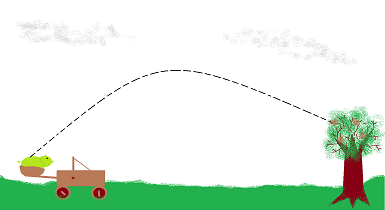
\includegraphics[width=12cm]{conceptsmall}
\end{center}

\chapter{Tehnologija}
\section{Uvod}
Igra je napisana v Scali, z izjemo dela, ki generira drevesa -- ta je bil napisan v jeziku Clojure. Scala je razmeroma nov jezik, ki teče na JVM(Java Virtual Machine) in hkrati podpira objektno ter funkcijsko programiranje. Clojure je moderen dialekt Lispa, ki tudi teče na JVM. Pred začetkom projekta sva bila čista začetnika v obeh jezikih -- sedaj Jaka zna nekaj Clojura in Matic nekaj Scale.\pa

Za grafiko sva uporabila knjižnico LWJGL. Prevedla in priredila sva
nekatere primere iz vaj. Igra ne uporablja naprednih tehnik in
funkcionalnosti OpenGL-a, predvsem zato, ker ima Matic precej počasen
prenosnik in za nameček na njem poganja Linux, ki ne podpira njegove
vgrajene grafične kartice. Grafika mu teče v programsko-pospešenem
načinu. (To ni le šala, ampak je bil dejansko precej velik faktor pri nekaterih
odločitvah)

\section{Prevajanje}
Prvi problem na katerega sva naletela je, kako hkrati prevajati Scalo in Clojure, ter kako v Scali uporabiti funkcije iz Clojura. Oba jezika sta v precejšnji meri kompatibilna z Javo, v smislu, da lahko uporabljata vse Javine razrede, z nekaj truda gre tudi obratno, z še nekaj več truda, pa lahko sodelujeta tudi Scala in Clojure.\pa

Po približno tednu pisanja lastne skripte za prevajanje, ki sva jo poimenovala ``bashbeans'', sva ugotovila, da za oba jezika obstaja način, za dinamično nalaganje kode med delovanjem programa. Tako se mora prevesti le del, ki je v Scali, ta pa nato dinamično naloži Clojure datoteke. Pri tem je nekaj slabosti glede razhroščevanja, ter hitrosti izvajanja, ampak je v primerjavi s prejšnjimi poskusi zelo enostavno.\pa

Delno vlogo pri razvoju bashbeans je imelo spet tudi dejstvo, da ima Matic precej počasen prenosnik, ter da ima Scala zelo počasen prevajalnik -- bashbeans tako vsakokrat shrani MD5 hash vrednosti izvornih datotek in ne prevaja ponovno tistih datotek, ki se niso spremenile.\pa

Kasneje sva odkrila, da ima Scala tudi fsc(fast scala compiler), ki naloži prevajalnik v ozadje kot daemon in tudi hrani delno prevedene datoteke in je tako le prvo prevajanje po zagonu sistema počasno. Tako je na žalost večina uporabnosti bashbeansa odpadla, imava pa še dovolj idej, kako ga poboljšati in morda uporabiti še na kakem drugem projektu.

\section{Modeliranje}
Zelo zgodaj v razvoju sva se odločila, da bodo vsi modeli generirani programsko -- nekateri so tako skorajda ročno zapisani v kodi, kar ni najlepše, ampak večina pa uporablja nekakšne naključne algoritme za generiranje. Tu gre posebej poudariti generiranje dreves, kateremu je naprej v dokumentaciji posvečen precej dolg odsek.\pa

Pri generativnem pristopu se je funkcijsko programiranje zelo izkazalo, saj je možno npr. napisati razred, ki v konstruktor sprejme dve funkciji: eno ki generira objekte, ter drugo, ki iz zgeneriranih podatkov izriše grafiko -- razred nato znotraj sebe avtomatsko shrani izris kot OpenGL DisplayList in so tako nadaljni izrisi precej hitrejši, brez da bi bilo treba za to kaj posebej narediti.\pa

Pristop se je izkazal za dobrega tudi, ko sva lahko zelo hitro razvila avtomatsko prilagajanje stopnje detajlov, glede na hitrost računalnika -- ob spremembi stopnje detajlov, razredu preprosto povemo, naj posodobi svoj izris.

\section{Generiranje dreves}
Problem generiranja primerno realističnih dreves se je izkazal za
algoritemsko precej zanimivega. V namene seminarske naloge je bil
rešen ``iz nule'', čeprav je ta problem že dokaj raziskan v obliki
L-sistemov in verjetno še česa. Ampak to ni tako zabavno.

Osnovna postavka merjenja uspeha končnega algoritma je bila funkcijska
čistost, saj sem želel postaviti sistem, ki iz peščice začetnih
podatkov generira neskončno število različnih dreves. Realističnost je
parameter, ki ga je bilo malo težje meriti zato je umetniški vtis
končnega rezultata bolj subjektivna ocena, da so drevesa uspešno
zgenerirana kot pa neka številka. Ako bi že moral definirati kako
uspešno algoritem generira drevesa, porečem, da 7.

\subsection{Osnovni princip}
Algoritem je zasnovan kot generator fraktalov, ki mu podamo nek vektor
in osnovno dolžino veje, ta pa potem rekurzivno kliče samega sebe,
dokler ne doseže neke smiselno določene meje globine drevesa.

Glavna funkcija algoritma se najprej odloči koliko vej je potrebnih na
trenutni globini, kar je definirano z vrsto praštevil (2,3,5
...). Nato izračuna vektorski produkt med podanim vektorjem V in nekim
izmišljenim vektorjem, s čimer dobi prvo vejo na trenutnem nivoju.

Ko je izbrana prva veja, jo samo (N-1)-krat duplicira in zavrti okrog
vektorja V. Tako ima osnovno vejo (vektor V) ter N nanjo pravokotnih
vej, ki predstavljajo poddrevo in so enakomerno razporejene po ravnini
na vrhu V.

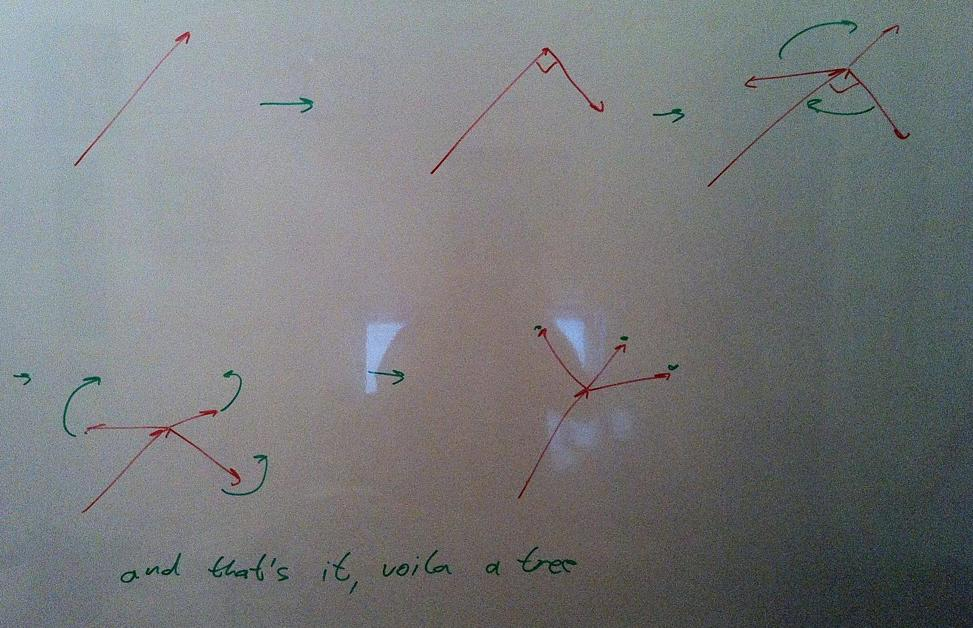
\includegraphics[width=12cm]{algorithmsketch.jpg}

Naslednji korak je samo še preprosta rotacija vseh vej za nek kot v
nasprotni smeri vektorja V in že imamo zgenerirano krošnjo za podano
vejo oz. deblo. Nato algoritem spet pokliče samega sebe na vrhu vsake
tako zgenerirane veje.


\subsection{Naključnost}
Po zgornjem algoritmu so drevesa sicer zgledala dokaj realistična,
vendar pa so bila vsa enaka, kar je bilo tako dolgočasno, kot je
onemogočalo, da bi tudi gozd deloval prilično resničen. Rešitev je
torej neka stopnja naključnosti.

Že intuitivno je opaziti, da drevo ne more biti popolnoma naključno,
saj potem izgubi na vsem kar ga sploh dela za drevo in postane samo
kup nekoherentnih črt. V interesu pravega znanstvenega pristopa in
izogibanja intuitivnim skokom logike, je bilo zgenerirano tudi eno
tako drevo.

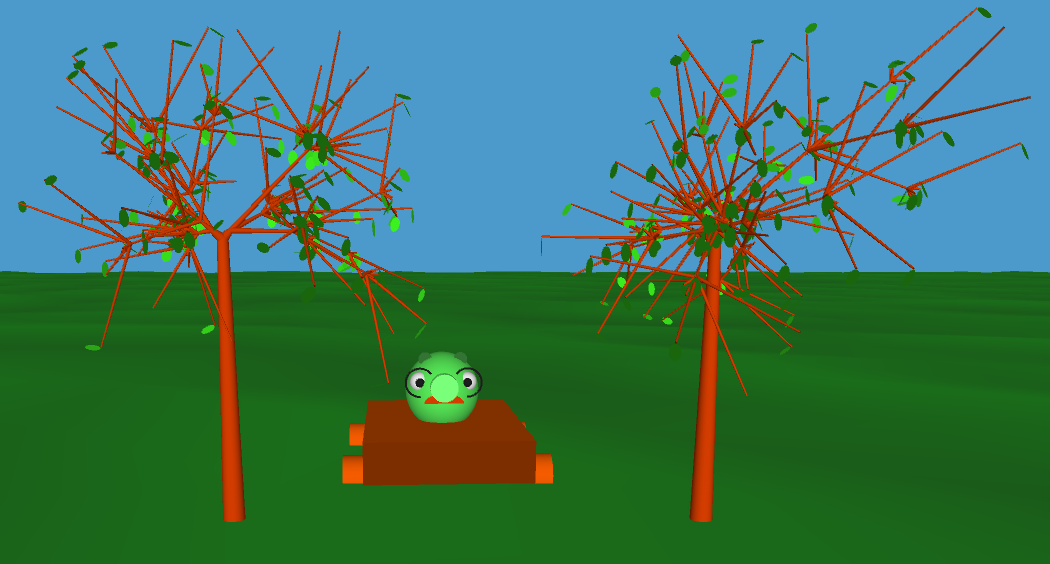
\includegraphics[width=12cm]{randomtree.png}

Naključnost je bilo zategadelj potrebno zapreti v neke smiselne
okvire, tako da bo algoritem sposoben generirati dovolj različnih
dreves, a bo vseeno vsakič zgeneriral drevo.

Podobno kot se osnoven algoritem izvaja v treh korakih, je tudi
naključnost dodana na tri osnovne načine.

Prva stopnja naključnosti se zgodi pri razporejanju vej po ravnini nad
osnovno vejo. Tu se pri vsaki rotaciji kotu preprosto doda nek
naključno izbran majhen kot v naključno smer, tako da razporeditev ni
čisto uniformna.

Druga stopnja naključnosti pride pri izbiri kota rotacije ``navzgor'',
ki določa kako široka bo krošnja. Tu gre za dokaj osnovno verzijo
uteženega naključnega izbiranja - algoritmu je namreč podan statično
izbran spisek deliteljev polnega radiana, tako da so naključne izbire
v končni fazi zgenerirale subjektivno zadvooljivo drevo. V končni
verziji kode ta del verjetno ne bo več tako statičen.

Najbolj zanimivo računanje naključnosti pa je pri izbiranju dolžine
vej, saj se je izkazalo za izredno pomembno, da so vse naslednje veje
krajše od prejšnjih, ter da se zelo kratke veje ne pripetijo prezgodaj
v drevesu. V ta namen je bila ustvarjena funkcija naključne izbire,
kateri lahko podamo funkcijo gostote verjetnosti. Na ta način
pridobimo popoln nadzor nad obliko verjetnosti.

Funkcija gostote verjetnosti, ki se je izkazala za najboljšo, je
zlepek, ki zagotavlja, da ima vsak naslednji nivo krajše veje od
prejšnjega, ter vsaki naslednji možni izbiri dolžine določi tretjino
verjetnosti prejšnje. (dolžine so namreč zaporedje vse manjših
večkratnikov osnovne dolžine, ki je parameter algoritma).

\subsection{Gravitacija}


\chapter{Rezultati}


\end{document}
